\documentclass[a4paper, 12pt]{article}
\usepackage[utf8]{inputenc}
\usepackage[T1,T2A]{fontenc}
\usepackage[a4paper, top=2cm, bottom=2cm, left=1cm, right=1cm, marginparwidth=1.75cm]{geometry}
\usepackage{graphicx}
\usepackage{amsmath}
\usepackage{indentfirst}
\usepackage[english, russian]{babel}
\usepackage[section,above,below]{placeins}
\usepackage[noend]{algorithmic}
\usepackage{amssymb}
\usepackage{amsfonts}
\usepackage{pdfpages}
\usepackage{xcolor}
\usepackage{hyperref}

\begin{document}
\section{Методы кластерного анализа}
\section{Иерархические алгоритмы}
\section{Расстояния между кластерами}

{\it Возможные расстояния}:
\begin{enumerate}
    \item \textbf{Расстояние "ближайшего соседа"} (одиночная связь): $$\rho_{\min}(K_i,K_j)=\min_{x_i \in K_i, x_j \in K_j} \rho (x_i,x_j).$$ Равно расстоянию между самыми ближними объектами кластеров.
    \item \textbf{Расстояние "дальнего соседа"} (полная связь):$$\rho_{\max}(K_i,K_j)=\max_{x_i \in K_i, x_j \in K_j} \rho (x_i,x_j).$$ Равно расстоянию между самыми дальними объектами кластеров.
    \item \textbf{Невзвешенное попарное среднее}: $$\rho_{\text{mean}}(K_i,K_j)=\text{mean}_{x_i \in K_i, x_j \in K_j} \rho (x_i,x_j).$$ Равно среднему между всеми парами расстояний.
    \item \textbf{Взвешенное попарное среднее}: $$\rho_{\text{mean2}}(K_i,K_j)=\text{mean}_{x_i \in K_i, x_j \in K_j} \rho (k_1 \cdot x_i,k_2 \cdot x_j) = \text{mean}_{x_i \in K_i, x_j \in K_j} \dfrac{k_1 x_i + k_2 x_j}{k_1+k_2}.$$ Равно среднему между всеми парами расстояний с учетом весов $k_1,k_2$, равных ёмкости кластеров.
    \item \textbf{Незвешенный центроидный метод}: расстояние между кластерами равно расстоянию между их центрами тяжести, где центр тяжести есть среднее арифметическое всех объектов в кластере: $$x_c = \dfrac{\sum_{i=1}^k 1 \cdot x_i}{k}= \text{mean}_{x_i \in K_i} (x_i)$$
    \item \textbf{Взвешенный центроидный метод}. Как я понял, это расстояние между центрами, но с учетом весов, как в пункте 4. Но вообще начиная с пункта 4 нигде нет формул, так что не факт, что они у меня правильные.
    \item \textbf{Метод Варда}. Целевой функцией является внутригрупповая сумма квадратов: $$\text{SS}=\sum_i \sum_{x_j \in K_i} \rho(x_j,x_i),$$
    где сумма берётся по всем кластерам, $x_i$ -- среднее по кластеру $K_i$. Объединение в кластеры на каждой итерации происходит так, чтобы увеличение этой функции было минимальным.
\end{enumerate}

\section{Процедуры эталонного типа}
Наряду с иерархическими методами кластеризации существуют итеративные ($k$-средних), суть которых заключается в следующем (возможны модификации):
\begin{enumerate}
    \item Среди объектов $x_i$ некоторым образом выбираются $k$ штук -- центры будущих кластеров.
    \item Объекты, не отнесённые к какому-либо кластеру, приписываются тому кластеру, до которого будет наименьшее расстрояние.
    \item Центры кластеров пересчитываются.
    \item Для всех точек пересматривается их принадлежность к кластеру.
    \item Пункты 3-4 повторяются, пока точки могут менять принадлежность.
\end{enumerate}
На этом сайте хорошо показано, как работает метод $k$-средних: \url{https://www.naftaliharris.com/blog/visualizing-k-means-clustering/}

\section{Методика дискриминантного анализа}
\section{Что характеризует Лямбда Уилкса?}
\section{Что показывают квадраты расстояний Махаланобиса?}
\section{Какое максимальное число канонических дискриминантных функций допустимо в дискриминантном анализе?}
\section{Какую информацию дают стандартизованные и структурные коэффициенты дискриминантной функции?}
\section{Опишите процедуру отбора переменных с помощью стандартизованных и структурных коэффициентов}
\section{Какова интерпретация канонического коэффициента корреляции?}
Общее число дискриминантных функций не превышает числа дискриминантных переменных и, по крайней мере, на единицу меньше числа групп. Степень разделения выборочных групп зависит от величины собственных чисел: чем больше собственное число, тем сильнее разделение. Наибольшей разделительной способностью обладает первая дискриминантная функция, соответствующая наибольшему собственному числу $\lambda_i$, вторая обеспечивает максимальное различение после первой и т. д. Различительную способность $i$-й функции оценивают по относительной величине в процентах собственного числа  $\lambda_i$ от суммы всех  $\lambda$.

\textbf{Коэффициент канонической корреляции}. Другой характеристикой, позволяющей оценить полезность дискриминантной функции является коэффициент канонической корреляции  $r_i$. Каноническая корреляция является мерой связи между двумя множествами переменных. Максимальная величина этого коэффициента равна 1. Будем считать, что группы составляют одно множество, а другое множество образуют дискриминантные переменные. Коэффициент канонической корреляции для $i$-й дискриминантной функции определяется формулой: $$r_i = \sqrt{\dfrac{\lambda_i}{1+\lambda_i}}.$$

\textbf{Чем больше величина  $r_i$, тем лучше разделительная способность дискриминантной функции.}

\section{В каком случае учет априорных вероятностей может сильно изменить результаты классификации?}
Априорные вероятности оказывают наибольшее влияние при перекрытии групп и, следовательно, многие объекты с большой вероятностью могут принадлежать ко многим группам. Если группы сильно различаются, то учет априорных вероятностей практически не влияет на результат классификации, поскольку между классами будет находиться очень мало объектов
\section{Методика факторного анализа}
\section{Суть задачи вращения общих факторов}
Задача вращения общих факторов решается с целью улучшения их {\it интерпретируемости}. Производится попытка достижения простой структуры, в которой каждая переменная характеризуется преобладающим влиянием какого–то одного фактора. Факторные нагрузки могут быть изображены в виде диаграммы рассеяния, на которой каждая переменная представлена точкой. Можно повернуть оси в любом направлении без изменения относительного положения точек. При этом действительные координаты точек, то есть факторные нагрузки, изменяются. 
\begin{figure}[h!]
    \center{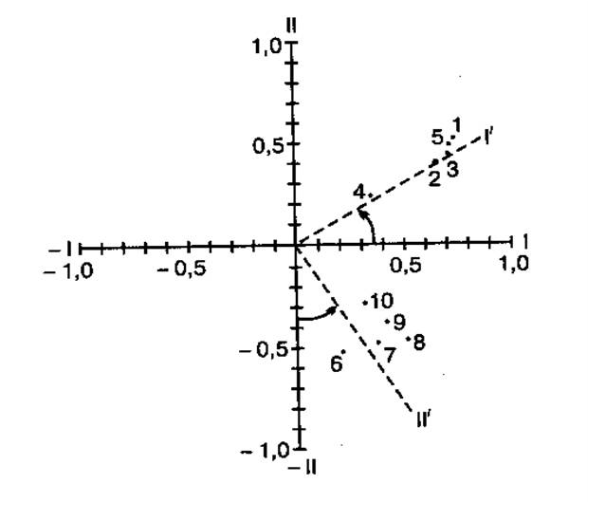
\includegraphics[width=0.5\linewidth]{rotate.png}}
    \caption{Зависимость сигнала от шума для данных.}
    \label{ris:image}
    \end{figure}

Существуют различные методы вращения факторов. Целью этих методов является получение понятной (интерпретируемой) матрицы нагрузок, то есть факторов, которые ясно отмечены высокими нагрузками для некоторых переменных и низкими -- для других. 

{\it Примеры методов вращения}:
\begin{itemize}
    \item­	\textbf{Варимакс}. Ортогональный метод вращения, минимизирующий число переменных с высокими нагрузками на каждый фактор. 
    \item ­	\textbf{Метод косоугольного (неортогонального) вращения}. Самое косоугольное решение соответствует дельте, равной 0 (по умолчанию). По мере того, как дельта отклоняется в отрицательную сторону, факторы становятся более ортогональными.
    \item ­	\textbf{Квартимакс}. Метод вращения, который минимизирует число факторов, необходимых для объяснения каждой переменной.
    \item ­	\textbf{Эквимакс}. Метод вращения, объединяющий методы варимакс, упрощающий факторы, и квартимакс, упрощающий переменные. Минимизируется число переменных с большими факторными нагрузками и число факторов, требуемых для объяснения переменной.
    \item ­	\textbf{Промакс-вращение}. Косоугольное вращение в предположении, что факторы могут коррелировать между собой. Оно производится быстрее, чем вращение типа косоугольного вращения, поэтому оно полезно для больших наборов данных.
\end{itemize}

\textbf{Примечание}. КОСОУГОЛЬНОЕ ВРАЩЕНИЕ --- такая трансформация факторного пространства, которая предполагает возможность проведения факторных осей под углами друг к другу, отличающимися от 90 градусов (от ортогональности)

\section{Критерий Кайзера}
\textbf{Критерий Кайзера или критерий собственных чисел}: отбираются только факторы с собственными значениями равными или большими 1. Это означает, что если фактор не выделяет дисперсию, эквивалентную, по крайней мере, дисперсии одной переменной, то он опускается. Этот критерий предложен Кайзером (Kaiser, 1960), и является, вероятно, наиболее широко используемым.
\section{Критерий Каменистой осыпи}
\section{Метод главных компонент}

\end{document}